\renewcommand{\thesection}{\arabic{chapter}.\arabic{section}}

\chapter*{General introduction: }
\addcontentsline{toc}{chapter}{General introduction}
\label{chap:intro}
\cleardoublepage
\doublespacing

\section*{The electricity markets and their modelisation over time}
\subsection*{Public utility pricing}

The interest for modelling the electricity markets can be traced back to the reference work by Marcel Boiteux, vice president in charge of economic studies at Electricité de France, at the outset of the second world war. The question at the time was mainly that of public utility pricing: in the context of a public monopoly, which price should the consumers face in order to allow the producers to recover their costs. \\

There are two main concerns that electricity producers have to face: the uncertainty of demand and the cyclicity of demand, for a commodity that essentially cannot be stored.\footnote{Electricity can be stored in hydroelectric dams, but the total energy stored is not enough to stabilize completely the demand faced by the other generation units, and only a fraction of the hydroelectric storage capacities can be actively replenished: the pumped storage facilities, which have two lakes and can therefore pump from the lower lake to the upper one on demand to store more electricity that that naturally stored in a lake that would be naturally replenished by a river.} \\

The first question is addressed in \cite{boiteux1951tarification}. In this paper, Boiteux considers a constant expected demand with fluctuations. The goal is to find the correct marginal pricing so that consumers internalize the additional cost that an uncertain demand entails for the producer. With a certain probability that demand is above its expected value by a given amount, how much more reserve capacity has to be kept in order to insure an accepted failure probability.\footnote{In the context of electricity, as production has to match demand at every point in time, every national grid is built with the notion of an acceptable probability of mismatch which translates in curtailments}\\

The second question is addressed in \cite{boiteux1960peak}. Contrary to the previous situation, demand is now considered to change over time in a deterministic and cyclical fashion. The question is to price electricity in order for consumers to be sensitive to the additional investment cost implied by higher demand peaks. \\

These contributions have sparked a larger litterature on the question of the pricing of economically non-storable commodities whose demand varies periodically, first in \cite{brown1969public} which studies the impact of stochastic demand on expected welfare. We refer the interested reader to the following review \cite{crew1995theory}. \\ 

This litterature has been mainly interested in questions of optimal pricing when the agent choosing the pricing tries to maximize the consumer's welfare, that is in the case of public monopolies. \\

\subsection*{Regulatory evolution}
The previous litterature took as an assumption the fact that these commodities were produced by public monopolies. Network utilities, such as gas, telecoms and electricity were thought to require to be organised as vertically integrated monopolies. \\

This view started to change in the 80s, with pressure to create competition. In 1984, access to gas pipelines was opened to competition in the USA and in 1990 Britain privatised electricity, separating generation and transmission. It was indeed thought that the natural monopoly emerged from the network, and that by separating generation from the network, generation could be opened to competition. \\

The overall argument for liberalisation is that private competition is considered a safer road towards efficiency than regulation of a monopoly. In a situation of perfect competition, actors would be strongly incentivized for efficiency gains, and these gains would be transferred to consumers. As perfect competition is a very rare situation, a new branch of the litterature started to coalesce around the questions of modeling competition in the case of electricity markets \cite{newbery1997privatisation}. \\

This liberalization movement has been somewhat slowed down after the California crisis in the early 2000s \cite{jamasb2005electricity}, which mainly concentrated on wholesale electricity markets. Because of very little price responsiveness of demand there was very high fluctuations in price as well as shortages \cite{borenstein2002trouble}. In Europe, the European Commission has pushed with success for the continuation of the program of liberalisation and integration, and wholesale markets for electricity are now quite ubiquitous, without further instances of failure as in California. 

\subsection*{The markets for electricity}
The way the markets for electricity are organised stem from three main characteristics:
\begin{itemize}
\item Every generation unit is to be paid the same unit price given the outcome of the market.
\item The market has to reflect the changing demand for electricity.
\item The form of the bids has to allow them to cope with the uncertain nature of demand at the time of bidding.
\end{itemize}

These ingredients have pushed for the creation of hourly or half-hourly markets, where suppliers are asked to submit supply schedules for a set number of bids (generally every 24 hours, that is 24 or 48 supply schedules once a day depending on whether the bids are hourly or half-hourly). These supply schedules take the form of a set of monotonous price quantity pairs, that can be considered as forming step functions\footnote{as in the case of the England and Wales pool in the 1990s} or functions linear by parts.\footnote{where price-quantity pairs are considered to be joined by lines instead of steps, which is the case for the French electricity day-ahead market, as well as the UK day-ahead market (half-hourly). Both of these markets are exchanged through EPEX Spot as of 2017.}\\

In the 1980s, a theoretical push has been made to model competition in supply functions. The first occurences of this approach can be found in \cite{grossman1981nash} and \cite{hart1982imperfect}. They consider situations where producers compete in supply curves when facing a given demand curve. The main result is that such problems can be solved and one can obtain specifications for optimal strategies in supply functions, but that there exists a very large multiplicity of equilibria in this setting.\\

Around the same time, \cite{klemperer1986price} introduces a setting in which firms choose endogenously to compete either in quantity or prices. This too yields a large multiplicity of outcomes, but the key insight comes from the fact that this multiplicity is drastically reduced when uncertainty is introduced.\\

This insight brings along the seminal paper \cite{KM} which studies supply function competition under uncertainty. In this paper, it is shown that although there is still a continuum of equilibria, this continuum has a structure that can be studied when suppliers face an uncertain demand. In the rest of this thesis, we denote supply function equilibria as SFE. \\

The setting introduced by Klemperer and Meyer is then rapidly put to use in the context of electricity markets, where \cite{Newgreen} studies the competition in the British spot market through the SFE framework. \\

This use of SFE sparks some debate as to whether a smooth function approximation can or not capture the correct effects in markets which are largely at the time asking bidders to submit step functions: \cite{von1993spot} argue that step functions of finite length are different to continuous functions.\footnote{This debate is largely obsolete now that most of the market rules imply bids that are linear by parts and not step functions anymore.}\\

This approach is still considered relevant by a number of authors. However, the multiplicity of equilibria makes it difficult to obtain clear results. In addition, the solutions are not exactly actionable, these functions being defined as solutions to a differential equation, therefore without an analytical formula. To overcome this issue, a number of authors either consider competition in simpler settings, for example Cournot competion settings applied to the electricity market in the case of \cite{borenstein1999empirical}, or choose to restrict themselves to one special solution out of the continuum of possible solutions that come out of the SFE framework: the supply function that is the unique linear solution out of this continuum. In so doing these authors pick arbitrarily one solution with a functional form and then use it to further analyze some economic questions. For example, \cite{green1996increasing} focuses on the linear supply solution out of the SFE multiple equilbria in order to have analytical tractable forms and study the effect of three different policies on competition, where 
\cite{hobbs2000strategic} is able to model transmission constraints with an affine supply function.\\

Overall, we refer the interested reader to the review by \cite{ventosa2005electricity} for a more detailed overview. In this thesis we rely heavily on the work by Klemperer and Meyer, and comment and contrast their results to ours. In order to make this easier to follow, we summarize in the following section the results of their paper that will be used in this thesis.

\section*{Klemperer and Meyer 1989}
Consider a setting in which firms bid supply functions while facing an uncertain demand. \\

Let $D(p,\theta)$ be the demand function as a function of demand shock $\theta$. Consider that for all $(p,\theta)$, $-\infty<D_p<0$, $D_{pp}\leq 0$ and $D_\theta>0$.\\

All firms are considered to be facing the same cost function $C(\cdot)$, with $C'(q)>0$ and $0<C''(q)<\infty$ for all $q>0$.\\

The timing is such that suppliers have to bid simultaneously a supply function prior to the realisation of demand shock $\theta$ being known. Consider for now two firms $i$ and $j$ with $S^k(p)$ the supply function of supplier $k$ and that these supply functions are twice differentiable. After this shock is known, every firm produces quantity $S^k(p^*(\theta))$ at price $p^*(\theta)$, such that $D(p^*(\theta)) = S^i(p^*(\theta)) + S^j(p^*(\theta))$.\\

Firm $i$'s residual demand is given by the total demand from which the supply of firm $j$ is subtracted, $D(p,\theta) - S^j(p)$. As $\theta$ is considered a scalar, the set of profit-maximizing points for every possible shock $\theta$ define a curve. If there is a unique intersection between $i$'s supply curve and the every possible demand curve, then such a supply curve is ex-post optimal, meaning that it is pointwise optimal for every realization of the shock $\theta$. \\

Given the assumption that supply curves indeed behave in this way, then maximizing the expected profit for the distribution of shocks can be abstracted away from the distribution of shocks, and $i$'s optimal supply curve solves for every shock $\theta$ the following program:

\begin{equation}\label{maxKM}
\max_p p\left( D(p,\theta) - S^j(p)\right) - C\left( D(p,\theta) - S^j(p)\right) 
\end{equation}

which F.O.C writes:

\begin{equation}\label{KMfoc}
\ D(p,\theta) - S^j(p) + \left( p - C^\prime\left( D(p,\theta) - S^j(p)\right)    \right)\left(  D_p(p,\theta)   - S^{j\prime}(p)\right) = 0
\end{equation}

with eq \ref{maxKM} being strictly concave in $p$ (we refer the reader to the original paper for more justifications), then eq \ref{KMfoc} defines the unique profit maximizing $p^*(\theta)$ for every $\theta$, which parametrizes the optimal supply function. \\

Consider that $D_{\theta p }=0$, that is that $\theta$ is an additive shock, and that we focus on symmetric equilibria, which allows us to drop the firms' superscripts. In addition, consider the fact that eq \ref{KMfoc} has to hold for every shock, it can therefore be rewritten as:
\begin{equation}\label{KMdiff}
S'(p) = \frac{S(p)}{p-C'(S(p))} + D_p(p)= f(p,S)
\end{equation}
This differential equation defines the supply function equilbria, the role of uncertainty being to ensure that this equation has to hold for every shock, therefore for every possible price. However, we can see that this differential equation is not accompanied by an initial condition. Therefore, there exists many adminissible solutions to this equation.\\

Supply functions are therefore bounded by possible values of their slope, namely that the functions have slopes bounded between $0$ and $+\infty$. By solving the differential equation, one can define the locus of points for which the solutions have slopes equal to these bounds, and thus obtain a region of admissible solutions, in the context of our problem:

\begin{figure}[h]
\centering
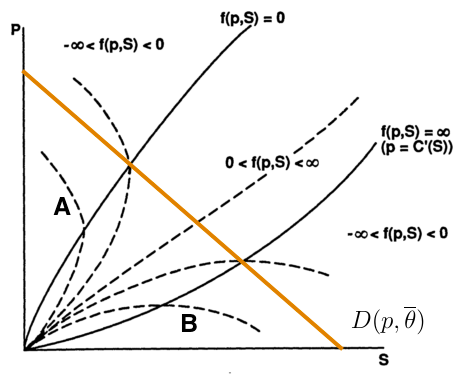
\includegraphics[width=8cm]{figintro/KMboundaries.png}
\caption{\small{This graph is adapted from the original paper by Klemperer and Meyer and illustrates the admissible region of solutions to the differential equation so as to verify the constraints on the slope of the supply function.}}
\label{KMboundaries}
\end{figure}

Therefore, the admissible set of solutions is defined by the upper bound of the demand shocks $\overline{\theta}$, in that if the solutions cross the slope boundaries before reaching the maximal shock, they cannot be accepted as solutions to the problem which constrains the solutions more strictly than the differential equation alone. In figure \ref{KMboundaries} the demand associated with the upper bound of the shocks $D(p,\overline{\theta})$ is represented in orange, and solutions A and B to the differential equation are not solutions to the problem as they reach the boundaries for smaller values of shocks.\\

The last result we will review here, is that in the case of an unbounded support of shocks, the set of equilibria is at its smallest, as it means that solutions have to have positive finite slope for every value of the shocks, and not only for a segment of the real line. \\

In some cases, for example for linear demand schedules, this set can collapse to a unique solution. \\

\section*{The case for ramping costs}

This framework models the costs as depending only on the quantity produced. In the context of electricity generation, an important type of costs that cannot be captured in such a specification of the cost function is that of ramping costs. These ramping costs refer to the fact that making production change over time induces specific costs.\\

To explain how such costs can arise, consider a thermal power plant (fossil fuels, nuclear etc.), and more precisely its core. Physically, to produce a given level of electricity, one has to maintain the core at a given temperature. To increase production, the temperature of the core has to increase. This means that when production is increased some fuel has to be lost to simply increase the temperature, this energy expenditure is not attached to any additional production.\\

This issue of ramping costs is at the heart of the choice of "quick" gas power plants to match sudden peaks in demand, where nuclear plants are more generally used for low frequency adjustments. Therefore these ramping costs are important technically on the electricity market. \\

Some papers have tried to estimate their values empirically, \cite{wolak2007quantifying} and more recently \cite{reguant2011welfare}. There is also a strand of litterature concerned with ramping costs, looking at the optimal price that allows to maximize the overall social welfare \cite{tanaka2006real}, that is, which price schedule allows to maximize the consumer welfare from which the production costs are substracted. This litterature does not use game-theoretical, but concerns itself with the best price signal to use in order to limit the ramping costs incurred due to varying demand, while still considering that the trajectory of demand is known. To our knowledge, there is no game-theoretical framework that has been brought to take ramping costs into account, and describe their effects on optimal strategies for the agents bidding on the market. 

\section*{Contribution}

This thesis focuses on the question of these ramping costs. In the first chapter, I tackle this question in a theoretical framework which yields predictions on the change of shape in supply functions over time as a function of the underlying uncertainty about demand shocks. The second chapter then introduces methods to study the shape of supply functions as observed on the French electricity market for data from 2011 to 2013, as well as methods to estimate the uncertainty contributed by the weather. The third chapter applies these methods to test these theoretical predictions on actual market data. The second and third chapters have been co-written with Henri de Belsunce, who finished his PhD in 2015 at the Munich-based Max Planck Institute for Innovation and Competition, under the supervision of Prof. Dr. Klaus M. Schmidt.\\

The first chapter focuses on what the introduction of ramping costs in a theoretical framework brings to the table. Our main contribution is to build and justify how these ramping costs can be tackled theoretically. First, we note that going to a continuous time descritption of the problem allows us to bring to the litterature about supply function equilibria powerful mathematical tools mostly used in option pricing, that is stochastic dynamics: we want to model ramping costs, i.e. costs associated to the variation in production, while retaining the key ingredient brought by \cite{KM}, i.e. the uncertainty, through the use of brownians, and more precisely, It\={o} processes. In so doing we face the issue that one cannot derive a brownian, and bring our second contribution, a physical argument about how power plants function that effectively operates as a low pass filter on our stochastic processes, and allow us to continue to build a tractable model of ramping costs under uncertainty. Third, we find in the litterature a specification of It\={o} processes that allows the model to remain tractable. \\

From these technical contributions we obtain our economic contributions in having a rich tractable model that yields results that contrast strongly with past results from the litterature. First, our solutions are unique, which contrasts with the usual continuum of Nash equilibria in the supply function equilibria litterature. Second, our solutions are not ex-post optimal, meaning that gathering information about the expected future evolution of demand yields different optimal strategies for suppliers, which in turn means that producers in our framework have a motive for submitting different supply functions from one time step to the next. Third, we have closed form solutions which yield specific predictions about the evolution of bids under uncertainty, namely that when uncertainty increase, suppliers submit steeper supply schedules in order to transmit more of these shocks to changes in price and not quantities, which are costly due to the existence of ramping costs. Finally, and less importantly, our framework justifies the existence of negative prices \footnote{Note that such negative prices happen, a few hours a year for example in France or Germany, for example in 2017 there were 146 such hours on 24 days in Germany \cite{epexnegP}} by producers being willing to pay consumers to consume more in order to avoid facing large variations in production, in contrast to everywhere positive schedules in the case of the supply function equilibria litterature.\\

In the rest of the thesis the goal is to test our predictions on data from the French day-ahead market. In so doing, as our theoretical predictions are mainly about the effect that the amount of uncertainty has on the slope of the optimal supply schedule, we separate the issue of building proxies for this uncertainty in our second chapter, and the actual analysis of the evolution of bids on these proxies in the third chapter.\\

In the second chapter our main focus is on analyzing our data, on building a way to describe it, and on building proxies for the uncertainty that producers face about the residual demand they have to anticipate when bidding on the day-ahead market. \\

First, we note that aggregate supply functions on the day ahead market cannot be well captured by parametric functions. Therefore we devise a way to describe them non-parametrically: we note that although they cannot be captured parametrically, they still have a rough S shape, and therefore four main parts, two extremal sections, and two interior ones separated by the inflection point of the curve in its middle secion. We define the transition points between these sections as the points of maximal absolute value for the derivative and second derivative of the supply schedules. This definition relies on kernel density estimates, and is therefore non-parametric. We observe that by using 5 such points, we are able to capture about 98\% of the intrisic variability of the supply schedules, and stop there although our method can be used to define more non parametric points. This method allows us to define points that we consider comparable across auctions, that allow use to perform cross-sectional analysis of our data in the third chapter. \\

Second, we build proxies for the amount of weather uncertainty that producers face and variables that capture information that suppliers have before bidding and should therefore be controlled for. For the information available to suppliers, we note that the effect of weather on the demand, and more importantly temperature, is well understood and that we need to control for it. To do so we build an effective temperature for France, as an average of the localised temperature weighted by the population of the spatial region considered, in order to capture the overall effect temperature has on heating.\footnote{France has a high level of electric heating overall, which means that demand for electricity is quite sensitive to temperature.} The rest of our focus is on building a proxy for the uncertainty concerning renewable production. To do so we analyze spatialized wind and sunlight data, and study it's spatial structure. We argue that spatial autocorrelation is a proxy for the uncertainty associated with weather forecasts, noting that if this data displays more spatial gradients, it is likely to be of a lesser quality due to the numerical nature of the weather simulations used to predict the weather, and therefore more uncertain.\\

Our contribution in the second chapter is to provide a non parametric way to define comparable points across auctions, and a measure of the uncertainty associated with weather forecasts.\\

In the third chapter, we focus on building the main proxy for the uncertainty faced by producers, and then on analyzing how the bids evolve relative to these proxies.\\

We note that the main uncertainty is about the shape of the demand schedules itself. Therefore we consider data available to the producers and regress the demand schedules on these variables. Next, we study the residuals of these regressions, and more specifically note that they are heteroskedastic. We leverage this, regressing the square of these residuals on our variables, in order to predict the expected amplitude of the residuals, that is the amplitude of the uncertainty of the demand schedule regression.\\

We then study the effect of our different proxies for uncertainty on the slope of the supply schedules, and note that if our proxies about the weather uncertainty (through the channel of renewable production) have the expected effect, the results are less clear cut for our residuals on the demand schedules. As we are working with full blown schedules in the quantity-price plane, we perform our residual analysis both on the prices and the quantities. We therefore obtain estimates for the uncertainty pertaining to the position of a given point of our demand schedule either in price or in quantity. In our theoretical framework, we make the strong assumptions that demand schedules are linear, and that demand shocks are additive, i.e. they do not impact the slope of the demand schedules. These assumptions yield that we cannot differentiate between shocks in price or quantity, and that they should have effects in the same direction: more uncertainty implying steeper supply curves to reduce the amount of fluctuations in production. However we observe that the effects of price and quantity uncertainty as estimated by our residuals' method yield opposite effects. Both of these assumptions, although required to obtain closed form results, are clearly not satisfied by our data, and we think that this is a clear path for improvement of the model.  \\

The contribution of the third chapter is to provide a way to estimate the uncertainty about the demand schedules faced by suppliers, and to estimate how this uncertainty affects the shape of the supply schedules at different points along its overall length, i.e. we provide a framework to describe how the functional form of schedules is affected by estimates of the uncertainty faced by suppliers.\\





 